\documentclass[aspectratio=169]{beamer}

\usetheme{default}
\usecolortheme{seahorse}
\setbeamertemplate{navigation symbols}{}
\setbeamertemplate{footline}[frame number]
\setbeamercovered{invisible}

\usepackage[utf8]{inputenc}
\usepackage{amsmath}
\usepackage{amssymb}
\usepackage{array}
\usepackage{tikz}
\usetikzlibrary{arrows.meta, positioning, shapes.geometric, fit, mindmap}

\tikzstyle{block} = [rectangle, draw, fill=blue!10, rounded corners,
  text width=2.1cm, minimum height=0.9cm, text centered, font=\scriptsize]
\tikzstyle{arrow} = [thick, -{Stealth[length=2mm]}]

\title[Image Signals \& Compression]{An Image Processing Workspace}
\subtitle{Signals, Transforms, and Compression: Concepts and Algorithms}
\author{}
\date{}

\begin{document}

% ------------------------------------------------------------
\begin{frame}[plain, label=titlepage]
  \begin{beamercolorbox}[wd=\textwidth,sep=1pt,rounded=true,shadow=true]{title}
    \centering
    \\[7pt]
    {\LARGE \bfseries Bindu}\\[7pt]
    An Image Processing Workspace \\[7pt]
    % \maketitle
  \end{beamercolorbox}

  \vspace{3.2em}
  \begin{center}
    \renewcommand{\arraystretch}{1.4}
    \newlength{\authorgap}
    \setlength{\authorgap}{1.0cm}
    \begin{tabular}{
        >{\centering\arraybackslash}p{0.25\textwidth}
        @{\hspace{\authorgap}}
        >{\centering\arraybackslash}p{0.25\textwidth}}
      { Sajiid Jawad Talukder} & { Proteek Rosul} \\
      { 2305041 } & { 2305042 }
    \end{tabular}
  \end{center}

  % \vspace{1.8em}
  % \begin{center}
  %   {\footnotesize\scshape CSE220 $\cdot$ CSE, BUET}
  % \end{center}
\end{frame}

% ------------------------------------------------------------
\begin{frame}{The Big Picture}
  \begin{itemize}
    \item An image is a 2D signal: analyze it, transform it, compact it.
    \item Every tool here is one of those three moves.
  \end{itemize}
  \vspace{0.3cm}
  \begin{columns}[t]
    \column{0.33\textwidth}
      \textbf{\small Analysis}
      \begin{itemize}\setlength\itemsep{5pt}
        \item[\scriptsize\textbullet] Color channel separation (R, G, B)
        \item[\scriptsize\textbullet] Per-channel and combined histograms
        \item[\scriptsize\textbullet] Luminance histogram
        \item[\scriptsize\textbullet] 2D FFT log-magnitude spectra
        % \item[\scriptsize\textbullet] Per-channel energy share
        \item[\scriptsize\textbullet] Color space comparison (RGB vs.\ YCbCr)
      \end{itemize}
    \column{0.33\textwidth}
      \textbf{\small Processing}
      \begin{itemize}\setlength\itemsep{5pt}
        \item[\scriptsize\textbullet] Gaussian and box blur
        \item[\scriptsize\textbullet] Laplacian sharpening
        \item[\scriptsize\textbullet] Unsharp masking
        \item[\scriptsize\textbullet] Per-channel or merged filtering
        \item[\scriptsize\textbullet] White scratch / dot removal
        % \item[\scriptsize\textbullet] Gaussian \& salt-and-pepper noise; median, Gaussian, NLM denoising
      \end{itemize}
    \column{0.33\textwidth}
      \textbf{\small Compression}
      \begin{itemize}\setlength\itemsep{5pt}
        \item[\scriptsize\textbullet] Partial image reconstruction from channel spectra
        \item[\scriptsize\textbullet] Fourier energy pruning (lossy)
        \item[\scriptsize\textbullet] PSNR \& MSE quality metrics
        % \item[\scriptsize\textbullet] Integer wavelet lifting (lossless)
        % \item[\scriptsize\textbullet] Pixel-exact round-trip verification
        % \item[\scriptsize\textbullet] Custom \texttt{.iwv} archive format
      \end{itemize}
  \end{columns}
\end{frame}


% ------------------------------------------------------------
\begin{frame}{Image as a 3D array}
  \begin{itemize}
    \item A colour image is a 3D array of shape $H \times W \times 3$.
    \item The third axis indexes the three colour channels.
  \end{itemize}
  \vspace{0.4cm}
  \begin{center}
  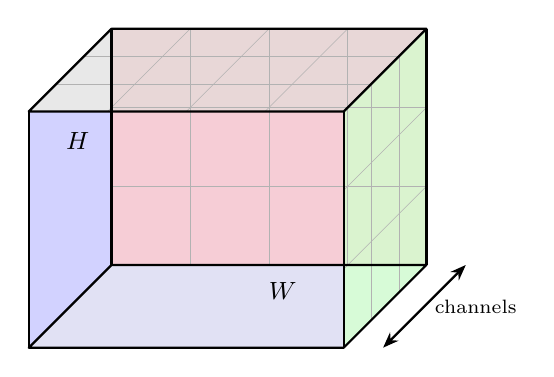
\begin{tikzpicture}[x={(-0.35cm,-0.35cm)}, y={(1cm,0cm)}, z={(0cm,1cm)},
                      line join=round]
    % Dimensions
    \def\W{4}  % width  (y)
    \def\H{3}  % height (z)
    \def\D{3}  % depth  (x) = 3 channels

    % Back face (x = \D)
    \fill[blue!25, opacity=0.7]
      (\D,0,0) -- (\D,\W,0) -- (\D,\W,\H) -- (\D,0,\H) -- cycle;
    % Bottom face
    \fill[gray!15, opacity=0.6]
      (0,0,0) -- (\D,0,0) -- (\D,\W,0) -- (0,\W,0) -- cycle;
    % Front face (x = 0)
    \fill[red!20, opacity=0.8]
      (0,0,0) -- (0,\W,0) -- (0,\W,\H) -- (0,0,\H) -- cycle;
    % Top face
    \fill[gray!30, opacity=0.6]
      (0,0,\H) -- (\D,0,\H) -- (\D,\W,\H) -- (0,\W,\H) -- cycle;
    % Right face (y = \W)
    \fill[green!20, opacity=0.7]
      (0,\W,0) -- (\D,\W,0) -- (\D,\W,\H) -- (0,\W,\H) -- cycle;

    % Grid lines on front face
    \foreach \zz in {0,...,\H}
      \draw[gray!60, very thin] (0,0,\zz) -- (0,\W,\zz);
    \foreach \yy in {0,...,\W}
      \draw[gray!60, very thin] (0,\yy,0) -- (0,\yy,\H);
    % Grid lines on top face
    \foreach \yy in {0,...,\W}
      \draw[gray!60, very thin] (0,\yy,\H) -- (\D,\yy,\H);
    \foreach \xx in {0,...,\D}
      \draw[gray!60, very thin] (\xx,0,\H) -- (\xx,\W,\H);
    % Grid lines on right face
    \foreach \zz in {0,...,\H}
      \draw[gray!60, very thin] (0,\W,\zz) -- (\D,\W,\zz);
    \foreach \xx in {0,...,\D}
      \draw[gray!60, very thin] (\xx,\W,0) -- (\xx,\W,\H);

    % Outer edges
    \draw[thick] (0,0,0) -- (\D,0,0) -- (\D,\W,0) -- (0,\W,0) -- cycle;
    \draw[thick] (0,0,\H) -- (\D,0,\H) -- (\D,\W,\H) -- (0,\W,\H) -- cycle;
    \draw[thick] (0,0,0) -- (0,0,\H);
    \draw[thick] (\D,0,0) -- (\D,0,\H);
    \draw[thick] (\D,\W,0) -- (\D,\W,\H);
    \draw[thick] (0,\W,0) -- (0,\W,\H);

    % Axis labels
    \node[font=\small] at (-0.5, \W/2, -0.5) {$W$};
    \node[font=\small] at (-0.2, -0.5, \H/2) {$H$};

    % Depth label
    \draw[{Stealth[length=2mm]}-{Stealth[length=2mm]}, thick]
      (0, \W+0.5, 0) -- (\D, \W+0.5, 0)
      node[midway, right, font=\scriptsize]{channels};
  \end{tikzpicture}
  \end{center}
  % \vspace{-0.1cm}
  % \begin{center}\scriptsize
  %   \texttt{img[row, col, 0]} = R \quad
  %   \texttt{img[row, col, 1]} = G \quad
  %   \texttt{img[row, col, 2]} = B
  % \end{center}
\end{frame}

% ------------------------------------------------------------
\begin{frame}{Channel Separation}
  \begin{itemize}
    \item Indexing the third axis extracts a single $H \times W$ plane.
    \item Each plane is a 2D array of intensities in [0, 255].
  \end{itemize}
  \vspace{0.4cm}
  \begin{center}
  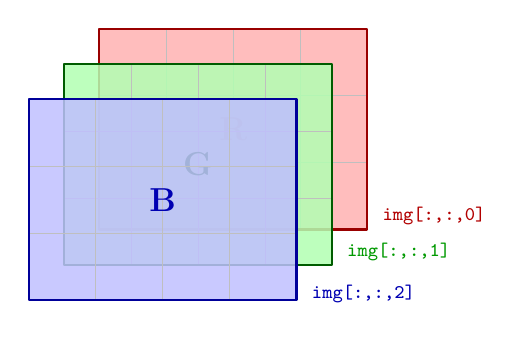
\begin{tikzpicture}[x={(-0.28cm,-0.28cm)}, y={(0.85cm,0cm)}, z={(0cm,0.85cm)},
                      line join=round]
    \def\W{4}
    \def\H{3}

    % Helper macro: draw one filled slice at depth \xx with given fill colour
    % Slices at x = 0 (R), 1 (G), 2 (B) — separated for clarity
    \foreach \xx/\fc/\lbl/\clr in {
        0/red!30/R/red,
        1.6/green!30/G/green!60!black,
        3.2/blue!25/B/blue}{
      % Fill
      \fill[\fc, opacity=0.85]
        (\xx,0,0) -- (\xx,\W,0) -- (\xx,\W,\H) -- (\xx,0,\H) -- cycle;
      % Grid
      \foreach \zz in {0,...,\H}
        \draw[gray!50, very thin] (\xx,0,\zz) -- (\xx,\W,\zz);
      \foreach \yy in {0,...,\W}
        \draw[gray!50, very thin] (\xx,\yy,0) -- (\xx,\yy,\H);
      % Border
      \draw[thick, \clr!60!black]
        (\xx,0,0) -- (\xx,\W,0) -- (\xx,\W,\H) -- (\xx,0,\H) -- cycle;
      % Channel label (centred on the face)
      \node[font=\large\bfseries, \clr!70!black] at (\xx, \W/2, \H/2) {\lbl};
    }

    % Annotation arrows pointing to each slice
    \node[font=\scriptsize, red!70!black]         at ( 0.0, \W+1, \H-2.8) {\texttt{img[:,:,0]}};
    \node[font=\scriptsize, green!60!black]       at ( 1.6, \W+1, \H-2.8) {\texttt{img[:,:,1]}};
    \node[font=\scriptsize, blue!70!black]        at ( 3.2, \W+1, \H-2.9) {\texttt{img[:,:,2]}};
  \end{tikzpicture}
  \end{center}
\end{frame}

% ------------------------------------------------------------
\begin{frame}{Histograms: Statistics of a Signal}
  \begin{itemize}
    \item Histogram = empirical distribution of pixel intensities.
    \item Luminance blends channels \emph{per pixel first}: $Y=0.299R+0.587G+0.114B$.
  \end{itemize}
  \vspace{0.3cm}
  \begin{center}
  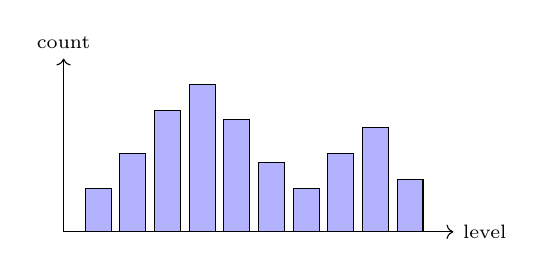
\begin{tikzpicture}[scale=0.55]
    \draw[->] (0,0) -- (9,0) node[right]{\scriptsize level};
    \draw[->] (0,0) -- (0,4) node[above]{\scriptsize count};
    \foreach \x/\h in {0.5/1.0, 1.3/1.8, 2.1/2.8, 2.9/3.4, 3.7/2.6, 4.5/1.6,
                        5.3/1.0, 6.1/1.8, 6.9/2.4, 7.7/1.2}
      \draw[fill=blue!30] (\x,0) rectangle +(0.6,\h);
  \end{tikzpicture}
  \end{center}
\end{frame}

% ------------------------------------------------------------
\begin{frame}{Frequency Content: The 2D FFT}
  \begin{itemize}
    \item Image $\rightarrow$ sum of 2D sinusoids of varying spatial frequency.
    \item \texttt{fftshift} centers DC; log-magnitude makes the spectrum viewable.
    \item Parseval's theorem: energy in space = energy in frequency.
  \end{itemize}
  \vspace{0.5cm}
  \begin{center}
  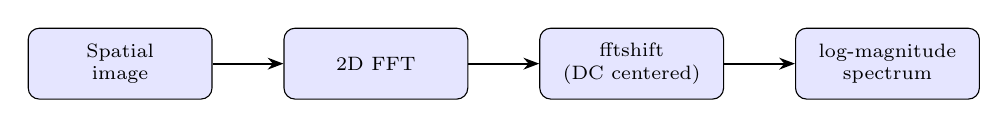
\begin{tikzpicture}
    \node[block] (img) {Spatial\\ image};
    \node[block, right=0.9cm of img] (fft) {2D FFT};
    \node[block, right=0.9cm of fft] (shift) {fftshift\\ (DC centered)};
    \node[block, right=0.9cm of shift] (log) {log-magnitude\\ spectrum};
    \draw[arrow] (img) -- (fft);
    \draw[arrow] (fft) -- (shift);
    \draw[arrow] (shift) -- (log);
  \end{tikzpicture}
  \end{center}
\end{frame}

% ------------------------------------------------------------
\begin{frame}{Partial Reconstruction}
  \begin{itemize}
    \item Inverse FFT is linear: rebuild from a subset of channel spectra.
    \item \emph{Phase}, not magnitude, carries most of the structure.
  \end{itemize}
  \vspace{0.3cm}
  \begin{center}
  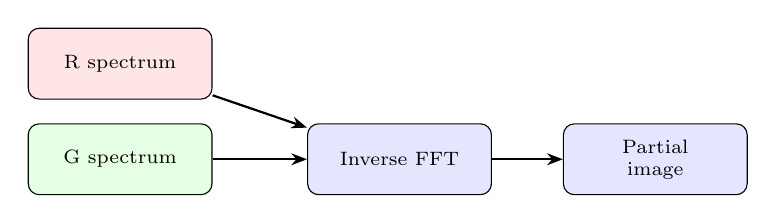
\begin{tikzpicture}
    \node[block, fill=red!10] (r) {R spectrum};
    \node[block, fill=green!10, below=0.3cm of r] (g) {G spectrum};
    \node[block, right=1.2cm of g] (ifft) {Inverse FFT};
    \node[block, right=0.9cm of ifft] (out) {Partial\\ image};
    \draw[arrow] (r) -- (ifft);
    \draw[arrow] (g) -- (ifft);
    \draw[arrow] (ifft) -- (out);
  \end{tikzpicture}
  \end{center}
\end{frame}

% ------------------------------------------------------------
\begin{frame}{Color Space: RGB vs.\ YCbCr}
  \begin{itemize}
    \item Linear change of basis: decorrelates brightness from color.
    \item $Y$ carries detail; $C_b,C_r$ are smooth $\Rightarrow$ energy compaction.
  \end{itemize}
  \vspace{0.3cm}
  \begin{center}
  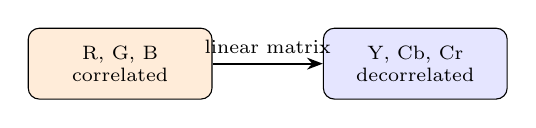
\begin{tikzpicture}
    \node[block, fill=orange!15] (rgb) {R, G, B\\ \scriptsize correlated};
    \node[block, right=1.4cm of rgb] (ycc) {Y, Cb, Cr\\ \scriptsize decorrelated};
    \draw[arrow] (rgb) -- node[above, font=\scriptsize]{linear matrix} (ycc);
  \end{tikzpicture}
  \end{center}
\end{frame}

% ------------------------------------------------------------
\begin{frame}{Spatial Filtering: Convolution}
  \begin{itemize}
    \item A kernel slides over the image; each pixel becomes a weighted local sum.
    \item Low-pass = blur (box, Gaussian); high-pass = sharpen (Laplacian, unsharp).
  \end{itemize}
  \vspace{0.3cm}
  \begin{center}
  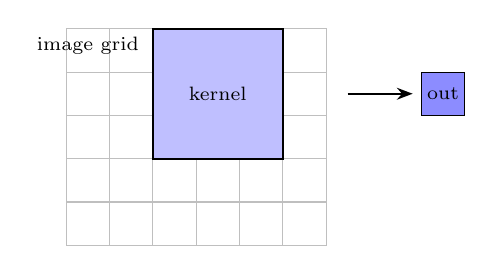
\begin{tikzpicture}[scale=0.55]
    \foreach \i in {0,...,5}
      \foreach \j in {0,...,4}
        \draw[gray!50] (\i,\j) rectangle +(1,1);
    \draw[thick, fill=blue!25] (2,2) rectangle +(3,3);
    \node at (3.5,3.5) {\scriptsize kernel};
    \node at (0.5,4.6) {\scriptsize image grid};
    \draw[arrow] (6.5,3.5) -- (8,3.5);
    \draw[fill=blue!45] (8.2,3) rectangle +(1,1) node[midway]{\scriptsize out};
  \end{tikzpicture}
  \end{center}
\end{frame}

% ------------------------------------------------------------
\begin{frame}{Lossy Compression: Fourier Energy Pruning}
  \begin{itemize}
    \item Rank frequency coefficients by energy; keep a target energy \%.
    \item Real images: conjugate-symmetric spectrum $\Rightarrow$ store half.
  \end{itemize}
  \vspace{0.3cm}
  \begin{center}
  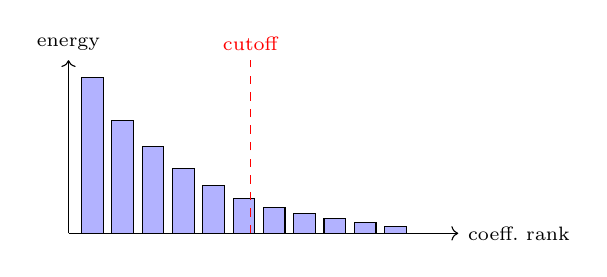
\begin{tikzpicture}[scale=0.55]
    \draw[->] (0,0) -- (9,0) node[right]{\scriptsize coeff.\ rank};
    \draw[->] (0,0) -- (0,4) node[above]{\scriptsize energy};
    \foreach \x/\h in {0.3/3.6, 1.0/2.6, 1.7/2.0, 2.4/1.5, 3.1/1.1,
                        3.8/0.8, 4.5/0.6, 5.2/0.45, 5.9/0.35, 6.6/0.25, 7.3/0.15}
      \draw[fill=blue!30] (\x,0) rectangle +(0.5,\h);
    \draw[dashed, red] (4.2,0) -- (4.2,4) node[above, font=\scriptsize]{cutoff};
  \end{tikzpicture}
  \end{center}
\end{frame}

% ------------------------------------------------------------

% ------------------------------------------------------------
\begin{frame}{Lossless Compression: Integer Wavelet Lifting}
  \begin{itemize}
    \item Integer Haar wavelets separate the image into averages and details.
    \item Keep every coefficient and compress the resulting patterns.
    \item Reverse the steps to recover the exact RGB image.
  \end{itemize}
  \vspace{0.5cm}
  \begin{center}
  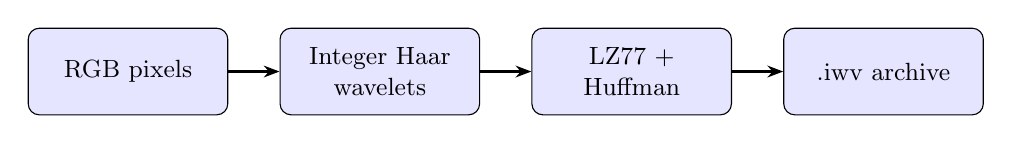
\begin{tikzpicture}
    \node[block, text width=2.3cm, minimum height=1.1cm, font=\small] (n0) {RGB pixels};
    \node[block, right=0.65cm of n0, text width=2.3cm, minimum height=1.1cm, font=\small] (n1) {Integer Haar\\wavelets};
    \node[block, right=0.65cm of n1, text width=2.3cm, minimum height=1.1cm, font=\small] (n2) {LZ77 +\\Huffman};
    \node[block, right=0.65cm of n2, text width=2.3cm, minimum height=1.1cm, font=\small] (n3) {.iwv archive};
    \draw[arrow] (n0) -- (n1);
    \draw[arrow] (n1) -- (n2);
    \draw[arrow] (n2) -- (n3);
  \end{tikzpicture}
  \end{center}
\end{frame}

% ------------------------------------------------------------
\begin{frame}{Photo Restoration}
  \begin{itemize}
    \item White top-hat subtracts the opened grayscale image to reveal bright marks.
    \item A repair mask selects the damaged areas.
    \item Inpainting estimates replacement colors from nearby pixels.
  \end{itemize}
  \vspace{0.5cm}
  \begin{center}
  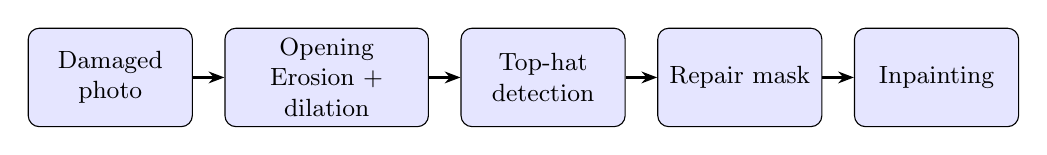
\begin{tikzpicture}
    \node[block, text width=1.85cm, minimum height=1.25cm, font=\small] (n0) {Damaged\\photo};
    \node[block, right=0.4cm of n0, text width=2.35cm, minimum height=1.25cm, font=\small] (opening) {Opening\\Erosion +\\dilation};
    \node[block, right=0.4cm of opening, text width=1.85cm, minimum height=1.25cm, font=\small] (n1) {Top-hat\\detection};
    \node[block, right=0.4cm of n1, text width=1.85cm, minimum height=1.25cm, font=\small] (n2) {Repair mask};
    \node[block, right=0.4cm of n2, text width=1.85cm, minimum height=1.25cm, font=\small] (n3) {Inpainting};
    \draw[arrow] (n0) -- (opening);
    \draw[arrow] (opening) -- (n1);
    \draw[arrow] (n1) -- (n2);
    \draw[arrow] (n2) -- (n3);
  \end{tikzpicture}
  \end{center}
\end{frame}

% ------------------------------------------------------------
\begin{frame}{Noise: Models and Denoising}
  \begin{itemize}
    \item Gaussian noise adds random variation; salt-and-pepper adds black or white dots.
    \item Median, Gaussian blur, or non-local means reduce noise.
    \item Denoising estimates a cleaner image and may soften some details.
  \end{itemize}
  \vspace{0.5cm}
  \begin{center}
  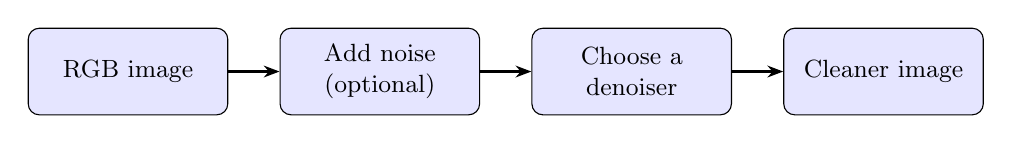
\begin{tikzpicture}
    \node[block, text width=2.3cm, minimum height=1.1cm, font=\small] (n0) {RGB image};
    \node[block, right=0.65cm of n0, text width=2.3cm, minimum height=1.1cm, font=\small] (n1) {Add noise\\(optional)};
    \node[block, right=0.65cm of n1, text width=2.3cm, minimum height=1.1cm, font=\small] (n2) {Choose a\\denoiser};
    \node[block, right=0.65cm of n2, text width=2.3cm, minimum height=1.1cm, font=\small] (n3) {Cleaner image};
    \draw[arrow] (n0) -- (n1);
    \draw[arrow] (n1) -- (n2);
    \draw[arrow] (n2) -- (n3);
  \end{tikzpicture}
  \end{center}
\end{frame}

% ------------------------------------------------------------
\begin{frame}{Recurring Threads}
  \begin{center}
  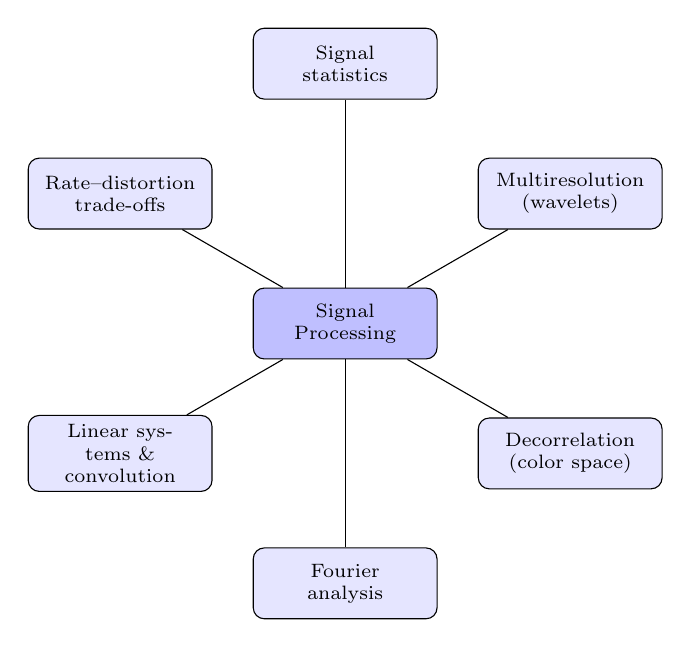
\begin{tikzpicture}[
      grow cyclic, shape=rectangle, rounded corners,
      level 1/.append style={level distance=3.3cm, sibling angle=60},
      every node/.style={block, fill=blue!10}]
    \node[fill=blue!25]{Signal\\ Processing}
      child{ node {Linear systems \&\\ convolution} }
      child{ node {Fourier\\ analysis} }
      child{ node {Decorrelation\\ (color space)} }
      child{ node {Multiresolution\\ (wavelets)} }
      child{ node {Signal\\ statistics} }
      child{ node {Rate--distortion\\ trade-offs} };
  \end{tikzpicture}
  \end{center}
\end{frame}

\end{document}